
\section{Population Level Analysis: Additive Faithfulness}
\label{sec:additivefaithful}

For a general regression function, an additive approximation may result in a
relevant variable being incorrectly marked as irrelevant. Such
mistakes are inherent in the approximation and may persist even in
the population setting.  In this section we give
examples of this phenomenon, and then show how the convexity
assumption
changes the behavior of the additive approximation. We work with $C=[0,1]^p$ as the support of the distribution in this section but all of our results apply to general hypercubes. We begin
with a lemma that characterizes the components of the additive approximation under mild conditions. 

% OLD lemma, requires product distribution
% \begin{lemma}
% \label{lem:general_int_reduction}
% Let $F$ be a product distribution on $\mathbf{C}=[0,1]^s$ with density function $p$ which is positive on $\mathbf{C}$. Let
% $X=(X_1,...,X_p) \sim F$. Let $f: \mathbf{C} \rightarrow \R$ be an
% integrable function.
% Let 
% \begin{equation}
% f_k^*, \mu^* \coloneqq \argmin_{f_1,\ldots, f_p, \mu} \Bigl\{ \E \bigl( f(X)  -
%  \sum_{k=1}^s f_k(X_k) -\mu \bigr)^2 
%         \,:\, \E f_k(X_k) = 0\Bigr\}.
% \end{equation}
% Then $\mu^* = \E f(X)$ and $f^*_k(x_k) = \E[ f(X) \given x_k] - \E f(X)$ and this solution is unique.
% \end{lemma}


\begin{lemma}
\label{lem:general_int_reduction}
Let $P$ be a distribution on $C=[0,1]^p$ with a positive density
function $p(\mathbf{x})$. Let $f: C \rightarrow \R$ be in $L^2(P)$. Let
\begin{align*}
f^*_1,...,&f^*_p, \mu^* \coloneqq  \\
&\arg\min \left\{ \E \Bigl( f(X) - \mu - \sum_{k=1}^p f_k(X_k)\Bigr)^2 \,:\,
f_k \in L^2(P),\, \E f_k(X_k) = 0,\; \forall k\right\}.
\end{align*}
With $\mu^* = \E f(X)$, 
\begin{equation}
\label{eq:backfit}
f^*_k(x_k) = \E\Bigl[ f(X) - \sum_{k' \neq k} f^*_{k'}(X_{k'}) \given
x_k\Bigr] - \E f(X), 
\end{equation}
and this solution is unique. 
\end{lemma}


Lemma~\ref{lem:general_int_reduction} follows from the stationarity
conditions of the optimal solution.   This result is known, and
criterion \eqref{eq:backfit} is used in the backfitting
algorithm for fitting additive models.   We include 
a proof as our results build on it.
% perhaps include this in an appendix??

\begin{proof}
  Let $f^*_1,...,f^*_p, \mu^*$ be the minimizers as defined; they exist since the set of mean zero additive functions is a closed subspace of $L^2(P)$.  We first
  show that the optimal $\mu$ is $\mu^* = \E f(X)$ for any $f_1, ...,
  f_k$ such that $\E f_k(X_k) = 0$. This follows from the stationarity
  condition, which states that $\mu^* = \E[ f(X) - \sum_k f_k(X_k)] =
  \E[ f(X) ]$. Uniqueness is apparent because the second derivative is
  strictly larger than zero and strong convexity is guaranteed.

  We now turn our attention toward the $f^*_k$s.  It must be that
  $f^*_k$ minimizes 
\begin{equation}
\min_{f_k} \E  \big( f(X) - \mu^* - \sum_{k' \neq k}
  f^*_{k'} (X_{k'}) - f_k (X_k) \big)^2 
\end{equation}
subject to $\E f_k(X_k) = 0$.
Fixing $x_k$, we will show that the value 
\begin{equation}
\E[ f(X) - \sum_{k' \neq k}
f_{k'}^*(X_{k'}) \given x_k] - \mu^*
\end{equation} 
uniquely minimizes
\begin{equation}
\min_{ f_k(x_k) } \int_{\mathbf{x}_{-k}} p(\mathbf{x}) 
         \Big( f(\mathbf{x}) - \sum_{k' \neq k} f^*_{k'} (x_{k'}) - f_k (x_k) -\mu^*\Big)^2 
                 d \mathbf{x}_{-k}.
\end{equation}
The first-order optimality condition gives us
\begin{align}
\int_{\mathbf{x}_{-k}} p(\mathbf{x}) f_k(x_k) d \mathbf{x}_{-k} &= 
  \int_{\mathbf{x}_{-k}} p(\mathbf{x}) 
      ( f(\mathbf{x})-\sum_{k' \neq k} f^*_{k'}(x_{k'})-\mu^*) d \mathbf{x}_{-k} \\  
p(x_k) f_k(x_k) &= \int_{\mathbf{x}_{-k}} p(x_k)
     p(\mathbf{x}_{-k} \given x_k ) 
     ( f(\mathbf{x}) - \sum_{k' \neq k} f^*_{k'} (x_{k'})-\mu^*) 
              d \mathbf{x}_{-k} \\
f_k(x_k) &= \int_{\mathbf{x}_{-k}} 
       p(\mathbf{x}_{-k} \given x_k ) 
     (f(\mathbf{x}) - \sum_{k'\neq k} f^*_{k'} (x_{k'})  -\mu^*) d \mathbf{x}_{-k} 
 \end{align}


To prove uniqueness, suppose $\tilde{f} = \sum_{j=1}^p \tilde{f}_j$ is
another additive function that achieves the same square error. Let
$\nu \in [0,1]$, and consider the expectation $\E\left( f(X) - \mu^* - (f^* + \nu
(\tilde{f} - f^*)) \right)^2$ as a function of $\nu$. The objective is
strongly convex if $\E (\tilde{f} - f^*)^2$, and so $\E( \tilde{f} -
f^*)^2 = 0$ by the assumption that $f^*$ and $\tilde{f}$ are both
optimal solutions. By Lemma~\ref{lem:additive_uniqueness}, we conclude
that $\E( f^*_j - \tilde{f}_j )^2 = 0$ as well and thus, $f^*_j =
\tilde{f}_j$ almost everywhere.

We note that $\E[ f(X) -\sum_{k'\neq k} f^*_{k'}(X_{k'}) | x_k] - \E
f(X)$ has mean zero as a function of $x_k$, which shows that the $f^*_k$s
are feasible.
\end{proof} 

In the case that the distribution in
Lemma~\ref{lem:general_int_reduction} is a product distribution, 
the additive components take on a simple form.

\begin{corollary}
\label{cor:product_int_reduction}
Let $p(\mathbf{x})$ be a positive density on $C=[0,1]^p$.
Let $\mu^*, f^*_k(x_k)$ be defined as in Lemma~\ref{lem:general_int_reduction}.
Then $\mu^* = \E f(X)$ and $f^*_k(x_k) = \E[ f(X) \given x_k] - \E f(X)$ and this solution is unique.
\end{corollary}

In particular, under the uniform distribution, $f^*_k(x_k) = \displaystyle\int f(x_k, \mathbf{x}_{-k}) d\mathbf{x}_{-k} - \int f(\mathbf{x}) d\mathbf{x}$.


\begin{example} Using Corollary~\ref{cor:product_int_reduction}, we
  give two examples of \emph{additive unfaithfulness} under the
  uniform distribution---where relevant variables are
  erroneously marked as irrelevant under an additive
  approximation. First, consider the following function:
\begin{equation}
f(x_1, x_2) = \sin( 2\pi x_1) \sin( 2 \pi x_2)\quad
\trm{(egg carton)} 
\end{equation}
defined for $(x_1, x_2) \in [0,1]^2$.  Then
$\displaystyle\int_{x_2} f(x_1, x_2) d x_2 = 0$ and
$\displaystyle\int_{x_1} f(x_1, x_2) d x_1 = 0$ for each $x_1$ and $x_2$. An additive approximation
would set $f_1 = 0$ and $f_2 = 0$.  Next, consider the function
\begin{equation}
f(x_1, x_2) = x_1 x_2 \quad \trm{(tilting slope)} 
\end{equation}
defined for $x_1 \in [-1,1],\; x_2 \in [0,1]$.  In this case
$\displaystyle\int_{x_1} f(x_1, x_2) d x_1 = 0$ for each $x_2$; therefore, we expect $f_2 = 0$ under the additive approximation. This function, for every fixed $x_2$, is a zero-intercept linear function of $x_1$ with slope $x_2$.
\end{example}

\begin{figure*}[htp]
\vskip-10pt
	\centering
	\subfigure[egg carton]{
		\centering
		{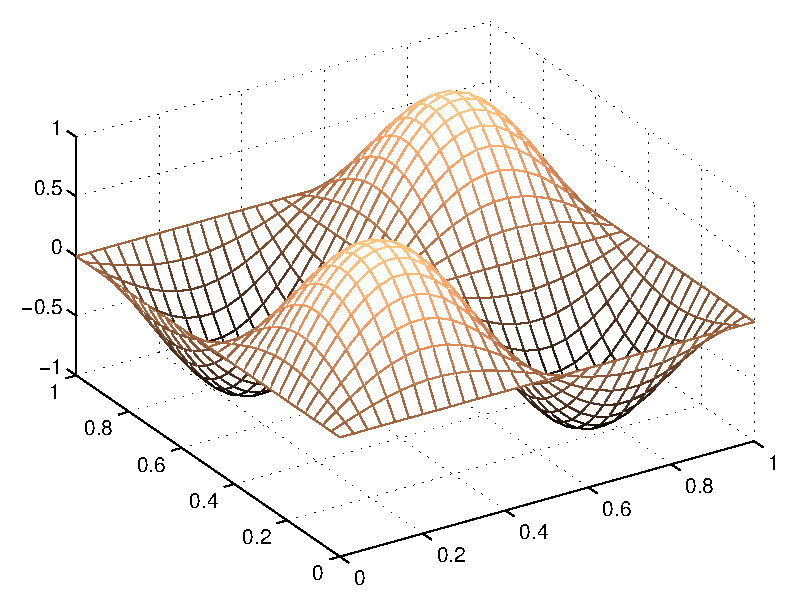
\includegraphics[width=0.4\textwidth]{figs/sine_wave_funct3}}
	}
	\subfigure[tilting slope]{
		\centering
		{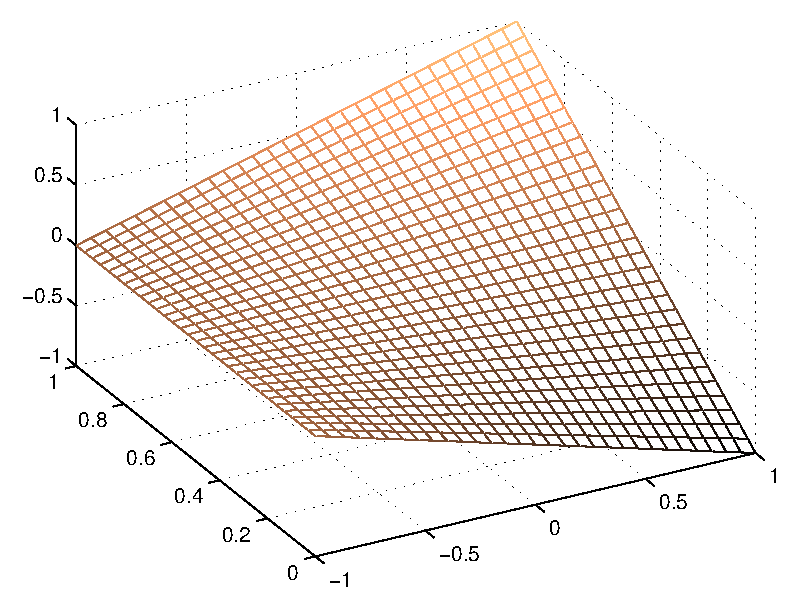
\includegraphics[width=0.4\textwidth]{figs/tilting_slope_funct3}}
	}
\caption{Two additively unfaithful functions. Relevant variables are
  zeroed out under an additive approximation because every ``slice''
  of the function integrates to zero.}
\vskip-10pt
\end{figure*}

In order to exploit additive models in variable selection, it is important to understand when the
additive approximation accurately captures all of the relevant variables.
We call this property \textit{additive faithfulness}. We first formalize the concept that a multivariate function $f$ \emph{does not depend on} a coordinate $x_k$.

\begin{definition}
%   Let $F$ be a distribution on $C=[0,1]^p$, and $f:C \rightarrow \R$. 
% We say that $f$ \textit{depends on coordinate $k$} if, for all $x_k \in [0,1]$, the set 
% $\big\{ x'_k \in [0, 1] \,:\, f(x_k, \mathbf{x}_{-k}) = f(x'_k, \mathbf{x}_{-k}) 
% \trm{ for almost all  $\mathbf{x}_{-k}$} \big\}$ 
% has probability strictly less than one.
% If $f$ is differentiable, then $f$ depends on $k$ if $\partial_{x_k} f \neq 0$ with probability greater than zero.
Let $C = [0,1]^p$ and let $f: C \rightarrow \R$. We say that $f$ \textit{does not depend on coordinate $k$} if for all $\mathbf{x}_{-k}$, $f(x_k, \mathbf{x}_{-k})$ is a constant as a function of $x_k$. If $f$ is differentiable, then $f$ does not depend on $k$ if $\partial_{x_k} f(x_k, \mathbf{x}_{-k})$ is 0 for all $\mathbf{x}_{-k}$.

In addition, suppose we have a distribution $P$ over $C$ and the additive approximation
\begin{equation}
\label{eqn:unconstrained_additive}
f_k^*, \mu^* \coloneqq \argmin_{f_1,\ldots, f_p, \mu} \Bigl\{ 
             \E \Bigl[\Bigl( f(X) - \sum_{k=1}^p f_k(X_k) -\mu \Bigr)^2 \Bigr]
         \,:\, \E f_k(X_k) = 0 \Bigr\}.
\end{equation}
We say that $f$ is \textit{additively faithful} under $P$ if
$f^*_k = 0$ implies that $f$ does not depend on coordinate $k$.
\end{definition}

% We can define the support $\trm{supp}(f) \coloneqq \{ k \,:\,
% \trm{$k$ is relevant to $f$}\}$. Let $f^* = \sum_{k=1}^p$, then $f$
% is additively faith if $\trm{supp}(f) = \trm{supp}(f^*)$.

Additive faithfulness is an attractive property because it implies
that, in the population setting, the additive approximation yields
a consistent variable screening.

\subsection{Additive Faithfulness of Convex Functions}

We now show that under a general class of distributions which we
characterize below, convex multivariate functions are additively
faithful. To simplify the presentation, we restrict our attention to
densities bounded away from $0/\infty$, that is, $0 < \inf
p(\mathbf{x}) \leq \sup p(\mathbf{x}) < \infty$.

\begin{definition}
\label{defn:boundary-point}
Let $p(\mathbf{x})$ be a density supported on $[0,1]^p$. We say that
$p(\mathbf{x})$ satisfies the \emph{boundary flatness condition} if
for all $j$ and for all $\mathbf{x}_{-j}$, 
\begin{enumerate}[(i)]
\item the derivatives $\frac{\partial
  p(\mathbf{x}_{-j} \given x_j)}{\partial x_j}, \frac{\partial^2
  p(\mathbf{x}_{-j} \given x_j) }{\partial^2 x_j}$ exist and are bounded,
for all $x_j \in [0,  \epsilon) \cup (1-\epsilon, 1]$ 
with $\epsilon > 0$ arbitrarily small,
\item for $x_j=0$ and $x_j=1$,
$\frac{\partial p(\mathbf{x}_{-j} \given x_j)}{\partial x_j}  =  
\frac{\partial^2 p(\mathbf{x}_{-j} \given x_j)}{\partial x_j^2} = 0$.
\end{enumerate}

\end{definition}

The boundary flatness condition intuitively states that two
conditional densities $p(\mathbf{x}_{-j} \given x_j)$ and
$p(\mathbf{x}_{-j} \given x_j')$ are similar when $x_j$ and $x_j'$ are
both close to the same boundary point. It is thus much more general
than requiring the density to be a product density. Boundary flatness
is a weak condition because it affects only an $\epsilon$-small region
around the boundary; $p(\mathbf{x}_{-j} \given x_j)$ can take
arbitrary shapes away from the boundary. Boundary flatness also allows
arbitrary correlation structure between the variables (provided
$p(\mathbf{x}) >0$). In Section~\ref{sec:boundary_flat}, we give a
detailed discussion of the boundary flatness condition and show
examples of boundary flat densities. In particular, we show that any
density supported on a compact set can be approximated arbitrarily
well by boundary flat densities.




% For instance, it is
% satisfied when the density is flat at the boundary of support---more
% precisely, when the joint density satisfies the property that
% $\frac{\partial p(x_j,\mathbf{x}_{-j})}{\partial x_j} =
% \frac{\partial^2 p(x_j, \mathbf{x}_{-j})}{\partial x_j^2} = 0$ at boundary
% points $x_j = 0, x_j=1$. The boundary flatness property is also
% trivially satisfied when $p$ is a product density.

The following theorem is the main result of this section.

\begin{theorem}
\label{thm:convex_faithful}
Let $p(\mathbf{x})$ be a density supported on $C=[0,1]^p$ and bounded
away from $0/\infty$ that satisfies the boundary flatness property.  
Suppose $f$ is a convex function with bounded second derivatives on an
open set containing $C$. Then $f$ is additively faithful under $p(\mathbf{x})$.
\end{theorem}

We let the domain of $f$ be slightly larger than $C$ for a technical
reason--it is so we can say in the proof that the Hessian of $f$ is
positive semidefinite even at the boundary of $C$.

% We give the full proof in Section~\ref{sec:faithful_proof} of the
% Appendix, but pause here to provide some intuition. 

We pause to give some intuition before we present the full proof.
Suppose that the underlying density is a product density.  We know
from Lemma~\ref{lem:general_int_reduction} that the additive
approximation zeroes out $k$ when, fixing $x_k$, every ``slice'' of
$f$ integrates to zero, but ``slices'' of convex functions that
integrate to zero cannot be ``glued together'' while still maintaining
convexity. Since the behavior of the whole convex function is
constrained by its behavior at the boundary, the same result holds
even if the underlying density is not a product density but merely
resembles a product density at the boundary, which is exactly the
notion formalized by the boundary flatness condition.

\begin{proof}

Fixing $k$ and using the result of
Lemma~\ref{lem:general_int_reduction}, 
we need only show that for all $x_k$, $ \E[ f(X) - \sum_{k'}
f_{k'}(X_{k'}) \given x_k] - \E f(X) = 0 $ 
implies that $f$ does not depend on coordinate $k$, i.e., 
$\partial_{x_k} f(\mathbf{x}) = 0$ for all $\mathbf{x}$.

Let us use the shorthand notation that $r(\mathbf{x}_{-k}) = \sum_{k'
  \neq k} f_{k'}(x_{k'})$ and assume without loss of generality that
$\mu^* = E[f(X)] = 0$. We then assume that for all $x_k$,
\begin{equation}
 \E[ f(X) - r(X_{-k})  \given x_k] \equiv 
 \int_{\mathbf{x}_{-k}}  p(\mathbf{x}_{-k} \given x_k ) 
 \big(f(\mathbf{x}) - r(\mathbf{x}_{-k}) \big) = 0.
\end{equation}
We let $p'(\mathbf{x}_{-k} \given x_k)$ denote 
$\frac{\partial p(\mathbf{\scriptstyle x}_{-k} \given x_k)}{\partial x_k}$ and 
$p''(\mathbf{x}_{-k} \given x_k)$ denote 
$\frac{\partial^2 p(\mathbf{\scriptstyle x}_{-k} \given x_k)}{\partial x_k^2}$ and
likewise for $f'(x_k, \mathbf{x}_{-k})$ and $f''(x_k,
\mathbf{x}_{-k})$. \\

We differentiate with respect to $x_k$ at $x_k = 0,1$ under the
integral. The details necessary to verify the validity of this
operation are technical and given in
Section~\ref{sec:dominated_condition} of the supplementary material.

\begin{gather}
\int_{\mathbf{x}_{-k}} p'(\mathbf{x}_{-k} \given x_k) 
\big( f(\mathbf{x}) - r(\mathbf{x}_{-k}) \big) + 
p(\mathbf{x}_{-k} \given x_k) f'(x_k, \mathbf{x}_{-k}) d \mathbf{x}_{-k}  = 0 
\label{eqn:integral1a} \\
\int_{\mathbf{x}_{-k}} p''(\mathbf{x}_{-k} \given x_k) 
\big( f(\mathbf{x}) - r(\mathbf{x}_{-k}) \big) 
   + 2 p'(\mathbf{x}_{-k} \given x_k) f'(x_k, \mathbf{x}_{-k}) \\
\nonumber \mbox{\ } +
p(\mathbf{x}_{-k} \given x_k) f''(x_k, \mathbf{x}_{-k}) d\mathbf{x}_{-k}  = 0 .
\end{gather}

By the boundary flatness condition, we have that $p''(\mathbf{x}_{-k}
\given x_k)$ and $p'(\mathbf{x}_{-k} \given x_k)$ are zero at $x_k =
x_k^0 \equiv 0$. The integral equations then reduce to the following:
\begin{align}
& \int_{\mathbf{x}_{-k}} p(\mathbf{x}_{-k} \given x^0_k) f'(x^0_k, \mathbf{x}_{-k}) d \mathbf{x}_{-k}= 0 \label{eqn:integral1b} \\
& \int_{\mathbf{x}_{-k}} p(\mathbf{x}_{-k} \given x^0_k) f''(x^0_k, \mathbf{x}_{-k}) d\mathbf{x}_{-k} = 0.
\end{align}
Because $f$ is convex, $f(x_k, \mathbf{x}_{-k})$ must be a convex
function of 
$x_k$ for all $\mathbf{x}_{-k}$. Therefore, for all $\mathbf{x}_{-k}$,
$f''(x^0_k, \mathbf{x}_{-k}) \geq 0$. Since $p(\mathbf{x}_{-k} \given
x^0_k) > 0$ by the assumption that $p(\mathbf{x})$ is a positive density, 
we have that $\forall \mathbf{x}_{-k}, f''(x^0_k, \mathbf{x}_{-k}) = 0$ necessarily.

The Hessian of $f$ at $(x^0_k, \mathbf{x}_{-k})$ then has a zero at
the $k$-th main diagonal entry. A positive semidefinite matrix with a
zero on the $k$-th main diagonal entry must have only zeros on the
$k$-th row and column; see proposition 7.1.10 of
\citet{HJ90}.  Thus, at all $\mathbf{x}_{-k}$, the
gradient of $f'(x^0_k, \mathbf{x}_{-k})$ with respect to
$\mathbf{x}_{-k}$ must be zero.
Therefore, $f'(x_k^0, \mathbf{x}_{-k})$ must be constant for all
$\mathbf{x}_{-k}$. By equation~\ref{eqn:integral1b}, we conclude 
that $f'(x_k^0, \mathbf{x}_{-k}) = 0$ for all $\mathbf{x}_{-k}$. We
can use the same reasoning for the case where $x_k = x_k^1$ and deduce
that $f'(x^1_k, \mathbf{x}_{-k}) = 0$ for all $\mathbf{x}_{-k}$. 

Because $f(x_k, \mathbf{x}_{-k})$ as a function of $x_k$ is convex, it must be that, for all $x_k \in (0,1)$ and for all $\mathbf{x}_{-k}$,
\begin{equation}
0 = f'(x_k^0, \mathbf{x}_{-k}) \leq f'(x_k, \mathbf{x}_{-k}) \leq 
    f'(x_k^1, \mathbf{x}_{-k}) = 0
\end{equation}
Therefore $f$ does not depend on $x_k$.
\end{proof}
% Now we apply the first-order condition of convex functions to any two points $(x_k, \mathbf{x}_{-k})$ and $(x'_k, \mathbf{x}_{-k})$ where $x_k, x'_k \in [0,1]$:
% \begin{align*}
% \forall \mathbf{x}_{-k}, f(x'_k, \mathbf{x}_{-k}) & \leq f(x_k, \mathbf{x}_{-k}) 
%   + f'(x_k, \mathbf{x}_{-k}) ( x'_k - x_k) \\ 
% f(x'_k, \mathbf{x}_{-k}) &\leq f(x_k, \mathbf{x}_{-k}) \\
% \forall \mathbf{x}_{-k}, f(x_k, \mathbf{x}_{-k}) & \leq f(x'_k, \mathbf{x}_{-k}) 
%   + f'(x'_k, \mathbf{x}_{-k}) ( x_k - x'_k) \\ 
% f(x_k, \mathbf{x}_{-k}) &\leq f(x'_k, \mathbf{x}_{-k})
% \end{align*}

% We thus have that $f(x_k, \mathbf{x}_{-k}) = f(x'_k, \mathbf{x}_{-k})$ for all $\mathbf{x}_{-k}$ and all pairs $x_k, x'_k \in (0,1)$. This proves that $f$ does not depend on $x_k$.

Theorem~\ref{thm:convex_faithful} plays an important role in our
finite sample analysis, where we show that the additive
approximation is variable screening consistent, even when the true function is not
additive.


\begin{remark}
  We assume twice differentiability in
  Theorems~\ref{thm:convex_faithful} to simplify the proof.  We
  expect, however, that this smoothness condition is not
  necessary---every convex function can be approximated arbitrarily
  well by a smooth convex function.
\end{remark}


\begin{remark} 
  We have not found natural conditions under which the opposite
  direction of additive faithfulness holds---conditions implying that if $f$ does not
  depend on coordinate $k$, then $f_k^*$ will be zero in the additive
  approximation.  Suppose, for example, that $f$ is only a
  function of $X_1, X_2$, and that $(X_1, X_2, X_3)$ follows a
  degenerate 3-dimensional distribution where $X_3 = f(X_1, X_2) -
  f^*(X_1) - f^*_2(X_2)$.  In this case $X_3$ exactly captures the
  additive approximation error.  The best additive
  approximation of $f$ would have a component $f^*_3(x_3) = x_3$ even
  though $f$ does not depend on $x_3$.
\end{remark}


\begin{remark}
In Theorem~\ref{thm:convex_faithful}, we do not assume a parametric
form for the additive components; the additive approximations may not
be faithful if we take a parametric form. For example, suppose we
approximate a mean-zero convex function $f(X)$ by a linear form $X
\beta$. The optimal linear function in the population setting is
$\beta^* = \Sigma^{-1} \trm{Cov}(X, f(X))$ where $\Sigma = \E X^\tran X$ is the
covariance matrix. Suppose the $X$'s are independent, centered, and have a
symmetric distribution with unit variance, and suppose $f(\mathbf{x})
= x_1^2 - \E[X_1^2]$. Then $\beta^*_1 = \E[ X_1 f(X)] = \E[ X_1^3 -
  X_1 \E[X_1^2]] = 0$.
\end{remark}

\subsection{Boundary Flatness Examples}
\label{sec:boundary_flat}

In this section, we give more examples of boundary flat densities (see
Definition~\ref{defn:boundary-point}) and discuss extending the notion
of boundary flatness to densities with a more general support. We
first start with a sufficient condition on the \emph{joint density}
that ensures boundary flatness.

\begin{example}
\label{ex:joint_density_flat}
Boundary flatness is satisfied if the joint density becomes flat at
the boundary. To be precise, let $p(\mathbf{x})$ be a joint density
bounded away from $0/\infty$ with a bounded second derivative.
Suppose also, for all $j$,
$$
\partial_{x_j} p(x_j,\mathbf{x}_{-j}) =
\partial_{x_j}^2 p(x_j, \mathbf{x}_{-j}) = 0\quad  \trm{at $x_j = 0, 1$}.
$$ It is then straightforward to show boundary flatness. One can first
verify that the derivatives of the marginal density $p(x_j)$ vanish
at $x_j = 0,1$ and then apply the quotient rule on
$\frac{p(x_j, \mathbf{\scriptstyle x}_{-j})}{p(x_j)}$ to show that $\partial_{x_j}
p(\mathbf{x}_{-j} \given x_j) = \partial_{x_j}^2 p(\mathbf{x}_{-j}
\given x_j) = 0$ at $x_j = 0,1$ as well.
\end{example}

The next example shows that any bounded density over a hypercube can
be approximated arbitrarily well by boundary flat densities.

\begin{example}
\label{ex:mixture_approx}
Suppose $p_\epsilon(\mathbf{x})$ is a bounded density over $[\epsilon,
  1-\epsilon]^p$ for some $0 < \epsilon < 1/2$. Let $q(\mathbf{x})$ be
an arbitrary boundary flat density over $[0,1]^p$ (one can take the
uniform density for instance). Define a mixture $p_{\lambda,
  \epsilon}(\mathbf{x}) = \lambda q(\mathbf{x}) + (1-\lambda)
p_\epsilon(\mathbf{x})$ where $0 < \lambda \leq 1$; then $p_{\lambda,
  \epsilon}(\mathbf{x})$ is boundary flat over $[0,1]^p$.

Now, let $p(\mathbf{x})$ be a bounded density over $[0,1]^p$. Let
$p_\epsilon(\mathbf{x})$ be the density formed from truncating
$p(\mathbf{x})$ in $[\epsilon, 1-\epsilon]^p$ and proper re-normalization. The corresponding
mixture $p_{\lambda,\epsilon}(\mathbf{x})$ then approximates
$p(\mathbf{x})$ when $\lambda$ and $\epsilon$ are both small.

Since $p_{\lambda,\epsilon}(\mathbf{x})$ remains boundary flat for
arbitrarily small $\epsilon$ and $\lambda$, $p(\mathbf{x})$ can be
approximated arbitrarily well (in $L_1$ for example) by boundary flat
densities.
\end{example}


% The result in Example~\ref{ex:joint_density_flat} further shows that boundary flat densities can arise from monotone marginal transformations of more general random vectors. This gives another way of approximating general densities by boundary flat densities.

% \begin{example}
% Let $X = (X_1,...,X_p)$ be drawn from a density supported on $[0,1]^p$, bounded away from $0/\infty$, and with a bounded second derivative. Let $\phi : [0,1] \rightarrow [0,1]$ be a monotonically increasing transformation. We will show that under certain conditions on $\phi$, the density of $(\phi(X_1), ..., \phi(X_p))$ is boundary flat.

% Suppose $\phi^{-1}$ has a bounded third derivative on some neighborhood around the boundary, say $[0, \epsilon) \cup (1-\epsilon, 1]$ and suppose $\phi^{-1\prime}(z) = \phi^{-1\prime\prime}(z) = \phi^{-1\prime\prime\prime}(z) = 0$ at $z=0,1$.

% Then, the density $p(z_1,...,z_p)$ of the transformed variables $z_j = \phi(x_j)$ is 
% $$ 
% p(z_1,...,z_p) = p_X(\phi^{-1}(z_1), ..., \phi^{-1}(z_p)) \prod_{j=1}^p \phi^{-1\prime}(z_j),
% $$ where $p_X(\cdot,...,\cdot)$ is the density of $X$.
% One can use the product rule and the chain rule to differentiate $p(z_1,...,z_p)$ and verify that $\partial_{z_j} p(\mathbf{z}) = \partial^2_{z_j} p(\mathbf{z}) = 0$ at $z_j = 0,1$ and thus show that $p(z_1,...,z_p)$ satisfies boundary flatness by Example~\ref{ex:joint_density_flat}.

% As a concrete example, we can use the following transformation $\phi_\epsilon$, defined in term of its inverse:
% $$\phi_\epsilon^{-1}(z) = \left\{ \begin{array}{cc} z^4 & \trm{if $z \leq \epsilon$} \\ 
%                      \frac{1-2\epsilon^4}{1-2\epsilon} z - \frac{ \epsilon + \epsilon^4}{1-2\epsilon} & \trm{if $\epsilon \leq z \leq 1-\epsilon$} \\
%                       1-(1-z)^4 & \trm{if $z \geq 1-\epsilon$} \end{array} \right.$$
% for any $1/2 > \epsilon > 0$. As $\epsilon$ becomes small, $\phi_\epsilon$ becomes close to the identity and so $(\phi_\epsilon(X_1), ..., \phi_\epsilon(X_p))$ closely approximates the original random variables $(X_1,...,X_p)$. Intuitively, $\phi$ stretches $X$ near the boundary so that a change in the transformed variable $z$ near the boundary corresponds to a much smaller change in original variable $x$. 
% \end{example}

In the discussion so far, we have restricted our attention to
densities supported and positive on the hypercube $[0,1]^p$ to
minimize extraneous technical details. It may also be possible to extend
the analysis to densities whose support is a convex and compact set so
long as the marginal density $p(x_j) > 0$ for all $x_j$ in the
support. A rigorous analysis of this however is beyond the scope of
this paper.

It may also possible to formulate a similar result to densities with
unbounded support, by using a limit condition $\lim_{|x_k| \rightarrow
  \infty} \frac{\partial p(\mathbf{\scriptstyle x}_{-k} \given
  x_k)}{\partial x_k} = 0$.  Such a limit condition however is not
obeyed by a correlated multivariate Gaussian distribution.  The next
example shows that certain convex functions are not additively
faithful under general multivariate Gaussian distributions.

\begin{example}
\label{examp:gaussian_counterexample}
Consider a two dimensional quadratic function $f( \mathbf{x}) = \mathbf{x}^\tran H \mathbf{x} + c$ with zero mean where $H = \begin{pmatrix} H_{11} & H_{12} \\ H_{12} & H_{22}\end{pmatrix}$ is positive definite and a Gaussian distribution $X \sim N(0, \Sigma)$ where $\Sigma = \begin{pmatrix}1 & \alpha \\ \alpha & 1 \end{pmatrix}$.
As we show in Section~\ref{sec:gaussian_example} of the supplementary
material \citep{supplement}, the additive approximation has the
following closed form.
\begin{align*}
f^*_1(x_1) &= \left( \frac{T_1 - T_2 \alpha^2}{1 - \alpha^4} \right) x_1^2 + c_1\\
f^*_2(x_2) &= \left( \frac{T_2 - T_1 \alpha^2}{1 - \alpha^4} \right) x_2^2 + c_2
\end{align*}
Where $T_1 = H_{11} + 2H_{12} \alpha + H_{22} \alpha^2$, $T_2 = H_{22}
+ 2H_{12} \alpha + H_{11} \alpha^2$, $c_1, c_2$ are constants such
that $f^*_1$ and $f^*_2$ both have mean zero. Let $H = \begin{pmatrix}
  1.6 & 2 \\ 2 & 5\end{pmatrix}$, then it is easy to check that if
  $\alpha = - \frac{1}{2}$, then $f^*_1 = 0$ and additive faithfulness
  is violated, if $\alpha > \frac{1}{2}$, then $f^*_1$ is a concave
  function. We take the setting where $\alpha=-0.5$, compute the
  optimal additive functions via numerical simulation, and show the
  results in Figure~\ref{fig:gaussian_example}.  Here $f^*_1$ is zero as
  expected.
\end{example}

Although the Gaussian distribution does not satisfy the boundary
flatness condition, it is possible to approximate the Gaussian
distribution arbitrarily well with distributions that do satisfy the
boundary flatness condition. We use an idea similar to that of
Example~\ref{ex:mixture_approx}.

\begin{example} 
\label{examp:boundaryflat_example}
Let $\Sigma$ be as in Example~\ref{examp:gaussian_counterexample} with
$\alpha = -0.5$ so that $f^*_1 = 0$. Consider a mixture $\lambda
U[-(b+\epsilon), b+\epsilon]^2 + (1-\lambda) N_b(0, \Sigma)$ where
$N_b(0,\Sigma)$ is the density of a \emph{truncated} bivariate
Gaussian bounded in $[-b, b]^2$ and $U[-(b+\epsilon), b+\epsilon]^2$
is the uniform distribution over a square. The uniform distribution is
supported over a slightly larger square to satisfy the boundary
flatness condition.

When $b$ is large, $\epsilon$ is small, and $\lambda$ is small, the
mixture closely approximates the Gaussian distribution but is still
additively faithful for convex
functions. Figure~\ref{fig:boundaryflat_example} shows the optimal
additive components under the mixture distribution, computed by
numerical integration with $b=5, \epsilon=0.3, \lambda=0.0001$. True
to our theory, $f^*_1$, which is zero under the Gaussian distribution,
is nonzero under the mixture approximation to the Gaussian
distribution. We note that the magnitude $\E f^*_1(X_1)^2$, although
non-zero, is very small, consistent with the fact that the mixture
distribution closely approximates the Gaussian distribution.
\end{example}


\begin{figure*}[t]
\vskip-10pt
	\centering
	\subfigure[Gaussian distribution]{
          \label{fig:gaussian_example}
		\centering
		{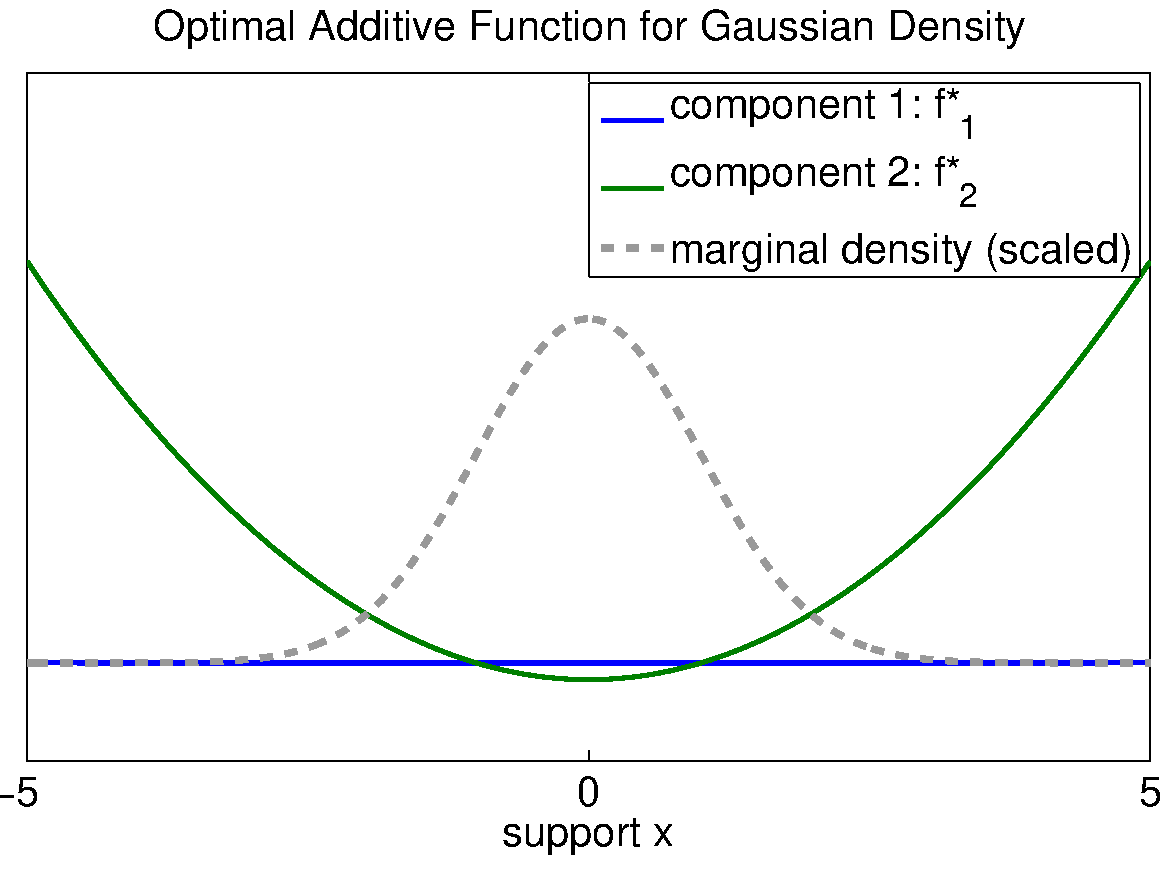
\includegraphics[width=0.4\textwidth]{figs/gaussian_example}}
	}
	\subfigure[Mixture approximation]{
          \label{fig:boundaryflat_example}
		\centering
		{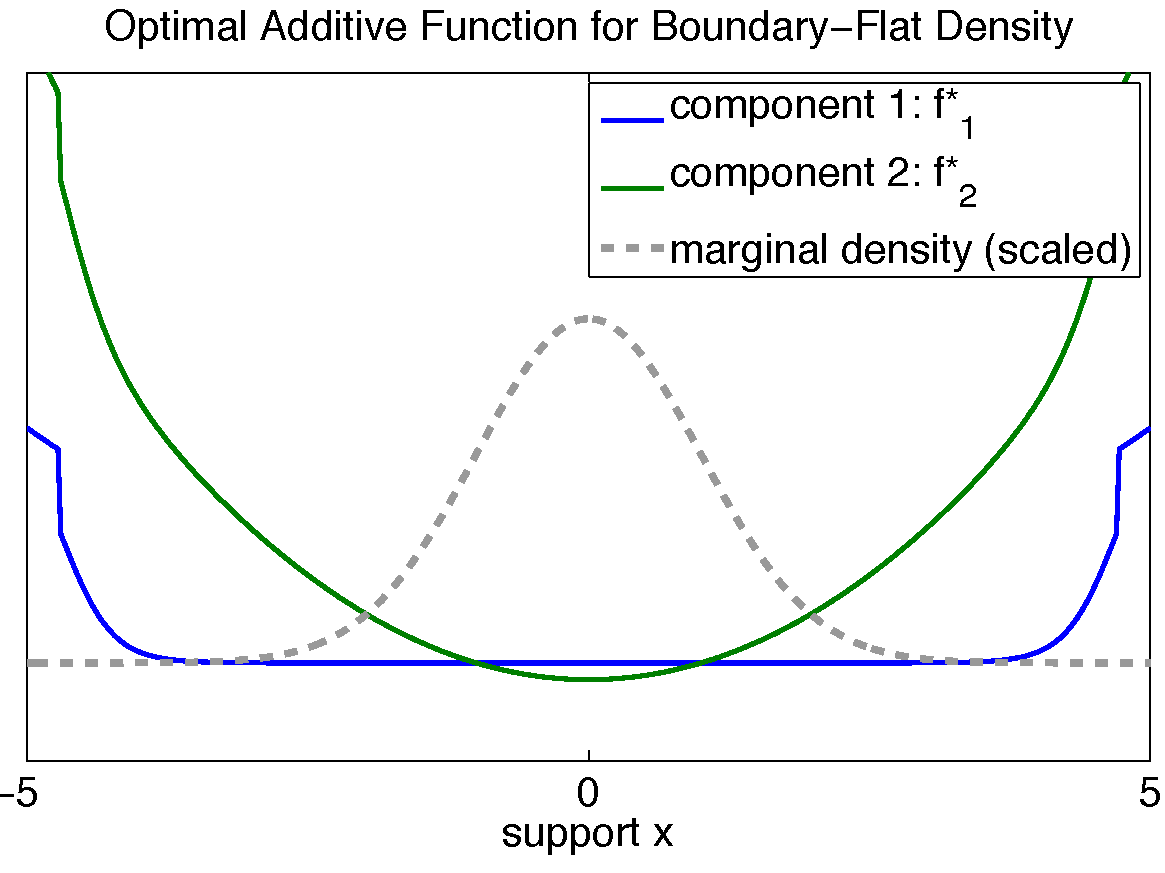
\includegraphics[width=0.4\textwidth]{figs/boundaryflat_example}}
	}
\caption{Optimal additive projection of the quadratic function
  described in Example~\ref{examp:gaussian_counterexample} under both
  the Gaussian distribution described in
  Example~\ref{examp:gaussian_counterexample} and the
  approximately Gaussian mixture distribution described in
  Example~\ref{examp:boundaryflat_example}. For the mixture
  approximation, we used $b=5, \epsilon=0.3, \lambda=0.0001$ where the
  parameters are defined in
  Example~\ref{examp:boundaryflat_example}. This example shows the
  effect and the importance of the boundary flatness condition.}
\vskip-10pt
\end{figure*}


\subsection{Convex Additive Models}

Although convex functions are additively faithful---under appropriate conditions---it is difficult to
estimate the optimal additive functions $f^*_k$s as defined in
equation~\eqref{eqn:unconstrained_additive}.  The reason is that $f^*_k$ need not be
a convex function, as Example~\ref{examp:gaussian_counterexample} and Example~\ref{examp:boundaryflat_example} 
show. It may be possible to estimate $f^*_k$ via smoothing, but we prefer an approach that is free of smoothing parameters. 
%The function $f^*_k$ can be shown to be smooth but it is preferable to use
%shape-constraints whenever possible to avoid the introduction of the
%additional smoothing bandwidth.
Since the true regression function $f$ is convex, we approximate the additive model with a \emph{convex} additive model. Without loss of generality, we assume in this section that $\E f(X) = 0$. 

We abuse notation and, for the rest of the paper, use the notation $f^*_k$ to represent convex additive fits:
%it is natural to ask when it is sufficient to estimate an convex additive model
\begin{equation}
\label{eqn:convex_additive}
\{ f^*_k \}_{k=1}^p = \arg\min \Big \{ 
    \E\Bigl( f(X) - \sum_{k=1}^p f_k(X_k) \Bigr)^2 \,:\, f_k \in \mathcal{C}^1, \, \E f_k(X_k) = 0 \Big \}
\end{equation}
where $\mathcal{C}^1$ is the set of univariate convex functions. 

If $p(\mathbf{x})$ is a product density, then $\E[ f(X) \given x_k]$
is convex in $x_k$ and the additive projection is simultaneously the
convex additive projection. Thus, in this case, additive faithfulness
trivially holds for the convex additive projection.  For a general
boundary flat density $p(\mathbf{x})$ however, the additive projection
need not be convex and we thus cannot say anything about additive
faithfulness of the convex additive projection.

Luckily, we can restore faithfulness by coupling the $f^*_k$s with a set of univariate concave fits on the \emph{residual} $f - f^*$:
\begin{equation}
\label{eqn:concave_postprocess}
g^*_k = \arg\min \Big\{
   \E\Bigl( f(X) - \sum_{k' \neq k} f^*_{k'}(X_{k'}) - g_k(X_k) \Bigr)^2
    \,:\, g_k \in \mh \mathcal{C}^1, \E g_k(X_k) = 0 
  \Big\}.
\end{equation}


\begin{theorem}
\label{thm:acdc_faithful}
Suppose $p(\mathbf{x})$ is a density on $C=[0,1]^p$ bounded away from
$0/\infty$ that satisfies the boundary flatness condition. Suppose
that $f$ is convex with a bounded second derivative on an open set
around $C$. Let $f^*_k$ and $g^*_k$ be as defined in equations
\eqref{eqn:convex_additive} and \eqref{eqn:concave_postprocess}, then
the $f^*_k$s and the $g^*_k$s are unique. Furthermore, $f^*_k = 0$
and $g^*_k = 0$ implies that $\partial_{x_k} f(\mathbf{x}) = 0$, that
is, $f$ does not depend on~$x_k$.
\end{theorem}

Before we can prove the theorem, we need a lemma that generalizes Theorem~\ref{thm:convex_faithful}.

\begin{lemma}
\label{cor:faithfulness_extension}
Suppose $p(\mathbf{x})$ is a density on $C=[0,1]^p$ bounded away from
$0$ and~$\infty$ satisfying the boundary flatness condition.  Let
$f(\mathbf{x})$ be a convex function with a bounded second derivative
on an open set around $C$. Let $\phi(\mathbf{x}_{-k})$ be a bounded
function that does not depend on $x_k$. Then the
unconstrained univariate function
 \begin{align}
h^*_k = \arg\min_{h_k} \mathbb{E} \Bigl[\bigl( f(X) 
           - \phi(X_{-k}) - h_k(X_k) \bigr)^2\Bigr]
\end{align}
is given by $h^*_k(x_k) = \mathbb{E}\bigl[ f(X) - \phi(X_{-k}) \,|\, x_k\bigr]$,
and $ h^*_k = 0$ implies that $\partial_{x_k} f(\mathbf{x}) = 0$.
\end{lemma}

\begin{proof}
  In the proof of Theorem~\ref{thm:convex_faithful}, the only property
  of $r(\mathbf{x}_{-k})$ we used was the fact that $\partial_{x_k}
  r(\mathbf{x}_{-k}) = 0$. Therefore, the proof here is identical to
  that of Theorem~\ref{thm:convex_faithful} except that we replace $r(\mathbf{x}_{-k})$ with $\phi(\mathbf{x}_{-k})$.
\end{proof}


\begin{proof}[Proof of theorem~\ref{thm:acdc_faithful}]

Fix $k$. Let $f^*_k$ and $g^*_k$ be defined as in
equation~\ref{eqn:convex_additive} and
equation~\ref{eqn:concave_postprocess}. Let $\phi(\mathbf{x}_{-k})
\equiv \sum_{k' \neq k} f^*_{k'}(x_{k'})$. Each $f^*_{k'}$ is convex
and thus continuous on $(0,1)$. The function $f^*_{k'}(x_{k'})$ is defined at
$x_{k'} = 0,1$; thus, $f^*_{k'}$ must be bounded and
$\phi(\mathbf{x}_{-k})$ is bounded.

We have that
\begin{align}
f^*_k &= \arg\min_{f_k} \Big\{
   \E\big( f(X) - \sum_{k' \neq k} f^*_{k'}(X_{k'}) - f_k \big)^2 
    \,:\, f_k \in  \mathcal{C}^1,\, \E f_k(X_k) = 0 
  \Big\} \\
g^*_k &= \arg\min_{g_k} \Big\{
   \E\big( f(X) - \sum_{k' \neq k} f^*_{k'}(X_{k'}) - g_k \big)^2 
    \,:\, g_k \in \mh \mathcal{C}^1,\, \E g_k(X_k) = 0 
  \Big\}
\end{align}

Let us suppose that $f^*_k = g^*_k = 0$. It must be then that
\begin{align*}
\argmin_{c \in \R} \E \left( f(X) - \phi(X_{-k}) - c (X_k^2 - m_k^2) \right)^2 = 0
\end{align*}
where $m_k^2 \equiv \E X_k^2$; this is because $c(x_k^2 - m_k^2)$ is either convex or concave in $x_k$ and it is centered, i.e. $\E[ X_k^2 - m_k^2] = 0$. Since the optimum has a closed form $c^* = \frac{\E\big[(f(X) -\phi(X_{-k}))(X_k^2 - m^2_k)\big]}{(\E X_k^2 - m^2_k)^2}$, we deduce that 
\begin{align*}
\E \big[ (f(X) - \phi(X_{-k})) (X_k^2 - m_k^2) \big] 
   &= \E[ (f(X) - \phi(X_{-k})) X^2_k] \\
&= \E[ \E[ f(X) - \phi(X_{-k}) \given X_k] X^2_k] = 0.
\end{align*}

We denote $h^*_k(x_k) = \E[ f(X) - \phi(X_{-k}) \given
  x_k]$.  Since $f(\mathbf{x})$ and $\phi(\mathbf{x}_{-k})$ are both bounded,
$h^*_k(x_k)$ is bounded as well. Therefore, $h^*_k$ is square
integrable and there exists a Fourier series $s_n(x_k)$ convergent to
$h^*_k$ in $L_2$. Since $p(\mathbf{x})$ is bounded, $$\lim_{n
  \rightarrow \infty} \E \left( s_n(X_k) - h^*_k(X_k ) \right)^2
\rightarrow 0$$ as well.

%Under the derivative continuity conditions in the theorem, we apply Lemma~\ref{lem:acdc_derivative_bound} in the appendix and know that $h^*_k(x_k)$ is twice-differentiable and has a second derivative bounded away from $-\infty$. Therefore, for a large enough positive scalar $\alpha$, $h^*_k(x_k) + \alpha(x_k^2 - m_k^2)$ has a non-negative second derivative and is thus convex.

If we can show that $\E h^*_k(X_k)^2 = 0$, we can apply
Lemma~\ref{cor:faithfulness_extension} and finish the proof. So let us
suppose for sake of contradiction that $\E h^*_k(X_k)^2 > 0$.

Let $0 < \epsilon < 1$ be fixed and let $n$ be large enough such that $\E( s_n(X_k) - h^*_k(X_k))^2 \leq \epsilon \E h^*_k(X_k)^2 $.
Since $s_n(x_k)$ is twice-differentiable and has a second derivative
bounded away from $-\infty$, there exists a positive scalar $\alpha$
such that $s_n(x_k) + \alpha(x_k^2 - m_k^2)$ has a non-negative second
derivative and is thus convex.

Because we assumed $f^* = g^* = 0$, it must be that
\[
\argmin_{c \in \R} 
\E\Big( f(X) - \phi(X_{-k}) - c\big( s_n(X_k) - \E s_n(X_k) + \alpha(X_k^2 - m_k^2)\big) \Big)^2 = 0
\]
This is because $c\big( s_n(x_k) - \E s_n(X_k) + \alpha(x_k^2 - m_k^2) \big)$ is
convex for $c \geq 0$ and concave for $c \leq 0$ and it is a centered
function.

Again, $c^* = \frac{\mathbb{E}[(f(X)-\phi(X_{-k}))\big( 
           s_n(X_k) - \E s_n(X_k)  + \alpha (X_k^2 - m_k^2) \big)]}{\mathbb{E}
       \big( s_n(X_k) - \E s_n(X_k) + \alpha (X_k^2 - m_k^2) \big)^2} = 0$, so
\begin{align*}
\mathbb{E}[ (f(X)-\phi(X_{-k}))& \big( s_n(X_k)- \E s_n(X_k) + \alpha
  (X_k^2-m_k^2) \big) ] \\
& = 
\mathbb{E}[ (f(X) - \phi(X_{-k})) s_n(X_k) ] \\
& = \mathbb{E}\Big[ \mathbb{E}[ f(X) - \phi(X_{-k}) \given X_k]  s_n(X_k) \Big] \\
& = \mathbb{E} h^*_k(X_k) s_n(X_k)  = 0
\end{align*}
where the first equality follows because $\E[ (f(X) - \phi(X_{-k})) (X_k^2 - m_k^2)] = 0$. \\

We have chosen $s_n$ such that $\E(h^*_k(X_k) - s_n(X_k))^2 \leq \epsilon \E h^*_k(X_k)^2$ for some $\epsilon < 1$. But, $\E (h^*_k(X_k) - s_n(X_k))^2 = \E h^*_k(X_k)^2 - 2 \E h^*_k(X_k)s_n(X_k) + \E s_n(X_k)^2 \geq \E h^*_k(X_k)^2$. This is a contradiction and therefore, $\E h^*_k(X_k)^2 = 0$.\\

Now we use
Lemma~\ref{cor:faithfulness_extension} with $\phi(\mathbf{x}_{-k}) =
\sum_{k' \neq k} f^*_{k'} (x_{k'})$ and conclude that
$f^*_k = 0$ and $g^*_k = 0$ together imply that $f$ does not depend on $x_k$.\\

Now we turn to uniqueness. Suppose for sake of contradiction that
$f^*$ and $\tilde{f}$ are optimal solutions to
(\ref{eqn:convex_additive}) and $\E (\tilde{f} - f^*)^2 > 0$.  $f^* +
\lambda ( \tilde{f} - f^*)$ for any $\lambda \in [0,1]$ must then also
be an optimal solution by convexity of the objective and
constraint. However, the second derivative of the objective $\E( f -
f^* - \lambda(\tilde{f} - f^*))^2$ with respect to $\lambda$ is $2 \E(
\tilde{f} - f^*)^2 > 0$. The objective is thus strongly convex and
$\E(f^* - \tilde{f})^2 = 0$. We now apply
Lemma~\ref{lem:additive_uniqueness} by letting $\phi_k = f^*_k -
\tilde{f}_k$. We conclude that $\E (f^*_k - \tilde{f}_k)^2 = 0$ for
all $k$. The uniqueness of $g^*$ is proved similarly.
\end{proof}


%%% JL:  I'm commenting out this proposition.  I don't see that it
%% serves any particular role in the rest of the paper.  Am I missing
%% something??
%%

% \begin{lemma}
% \label{lem:shape_approx_univariate}
% Let $C \subset \R^p$ be a compact set and let $h : C \rightarrow \R$. Let $p(x)$ be a positive density supported on $C$ and suppose $\E h(X) = 0$. Suppose that $\partial_{x_k} h(x)$, $\partial_{x_k} p( x \given x_k)$, and $\partial^2_{x_k} p( x \given x_k )$ are all continuous as functions on $C$. Suppose that $\partial^2_{x_k} h(x) \geq 0$.


% Let 
% \begin{align*}
% f^*_k(x_k) &= \arg\min_{f_k} \Big\{
%   \E \Big( h(X) - f_k(X_k) \Big)^2 \,:\, f_k \in \mathcal{C}^1,\, \E f_k = 0 \Big\} \\
% g^*_k(x_k) &= \arg\min_{g_k} \Big \{
%   \E \Big( h(X) - g_k(X_k) \Big)^2 \,:\, g_k \in \mh \mathcal{C}^1 ,\, \E g_k = 0 \Big\}
% \end{align*}
% be the best convex and concave univariate approximation respectively.\\

% Then, $f^*_k = 0$ and $g^*_k = 0$ iff $h^*_k(x_k) \equiv \E[ h(X) \given x_k ] = 0$.
% \end{lemma}

% \begin{proof}

% First, we establish that $h^*_k(x_k)$ is twice differentiable and that $\partial^2_{x_k} h^*_k(x_k)$ is lower bounded. 

% \begin{align*}
% h^*_k(x_k) &= \E[ h(X) \given x_k] \\
%  &= \int_{x_{-k}} h(x) p(\mathbf{x}_{-k} \given x_k) d \mathbf{x}_{-k}\\
% \partial^2_{x_k} h^*_k(x_k) 
%  &= \int_{\mathbf{x}_{-k}} h''(\mathbf{x}) p(\mathbf{x}_{-k} \given x_k) +
%  2 h'(x) p'(\mathbf{x}_{-k} \given x_k) + h(x) p''(\mathbf{x}_{-k} \given x_k) 
%  d\mathbf{x}_{-k} 
% \end{align*}

% The first term $h''(x) p(\mathbf{x}_{-k} \given x_k)$ is strictly positive. By assumption, the remaining terms are continuous and hence bounded on a compact set. $\partial^2_{x_k} h^*_k(x_k)$ is therefore lower bounded. Before proceeding, we also note that because $\E h(X) = 0$, it must be that $\E h^*_k(X_k) = 0$.

% Now suppose $f^*_k = 0$ and $g^*_k = 0$. Let $\sigma_k^2$ denote $\E X_k^2$. Then 
% \begin{equation}
% \arg\min_{c \in \mathbb{R}} \mathbb{E}\Big( h(X) - c (X_k^2-\sigma_k^2) \Big)^2 = 0
% \end{equation}
% Since optimal $c^* = \frac{\mathbb{E} [ h(X) (X_k^2-\sigma_k^2) ]}{\mathbb{E}[ X_k^2 ]}$, 
% we know $\mathbb{E} [ h(X) X_k^2 ] = 
% \mathbb{E} \Big[ \mathbb{E}[ h(X) \,|\, X_k] X_k^2 \Big] = 0$.\\

% Because $\partial^2_{x_k} h^*_k(x_k)$ is lower bounded, for large enough $\alpha$, $h^*_k(x_k) + \alpha (x_k^2 - \sigma_k^2)$ has a non-negative second derivative and thus is convex. Then
% \begin{equation}
% \arg\min_{c \in \mathbb{R}} \mathbb{E}\Big( h(X) 
%       - c (h^*_k(X_k) + \alpha (X_k^2 - \sigma_k^2)) \Big)^2 = 0
% \end{equation}
% Again, $c^* = \frac{\mathbb{E}[g(X)\big( 
%            h^*_k(X_k) + \alpha (X_k^2 - \sigma_k^2) \big)]}{\mathbb{E}
%        \big( h^*_k(X_k) + \alpha (X_k^2 - \sigma_k^2) \big)^2} = 0$, so
% \begin{align*}
% \mathbb{E}[ h(X) \big( h^*_k(X_k) + \alpha X_k^2 \big) ] &= 
% \mathbb{E}[ h(X) h^*_k(X_k) ] \\
% & = \mathbb{E}\Big[ \mathbb{E}[h(X) | X_k]  h^*_k(X_k) \Big] \\
% & = \mathbb{E} h^*_k(X_k)^2 = 0
% \end{align*}
% Therefore, $h^*_k(x_k) = 0$.

% \end{proof}
%%

% \begin{remark}
% Without restrictions on the distribution, a convex
%   function may not be additively faithful. Intuitively, an arbitrarily shaped
%   density $p$
%   may ``undo'' the convexity of $f$ so that the product
%   $p(\mathbf{x}) \, f(\mathbf{x})$ resembles an egg carton or a
%   tilting slope.  With appropriate conditions on the density $p$,
%   however, it is possible to relax the independence assumption.  We leave this to
%   future work.
% \end{remark}


% DO NOT CHANGE; RefTex variables -minx
 
%%% Local Variables: ***
%%% mode:latex ***
%%% TeX-master: "paper-submit.tex" ***
%%% End: ***

